\documentclass[11pt,a4paper]{ctexart}
\usepackage[margin=2.25cm]{geometry}
\usepackage{amsmath,amssymb,booktabs,array,longtable}
\usepackage{graphicx,float,xcolor}
\usepackage{hyperref}
\usepackage{enumitem}
\graphicspath{{figures/}}
\hypersetup{colorlinks=true,linkcolor=blue!55!black,urlcolor=blue!55!black}
\setlength{\parindent}{2em}
\setlength{\parskip}{0.25em}
\newcommand{\hpwl}{\operatorname{HPWL}}
\newcommand{\ov}{\operatorname{overflow}}
\newcommand{\code}[1]{\texttt{\detokenize{#1}}}

\title{精确非光滑 HPWL 的渐进合法化研究\\
\large 静电密度、混合对偶控制与 DREAMPlace 风格详细布局}
\author{HUAWEI\_EDA / DREAMPlace C++ 技术报告}
\date{2026 年 8 月 8 日}

\begin{document}
\maketitle

\begin{abstract}
本文研究一个严格不平滑 HPWL 的五阶段布局流程：先进行短时精确 HPWL 优化，再加入静电密度；随后以连续方式逐渐加入固定宏避障、行邻近和无障碍 segment 容量引导；最后执行 Greedy/Abacus 合法化和 DREAMPlace 风格合法后微调。所有全局布局的评价和接受判据均使用带 pin offset 的精确 HPWL，没有使用 weighted-average、log-sum-exp 等平滑线长代理。新增流程由 \code{--progressive-legalization} 显式开启，默认路径和原有调用方式不变。

在 ISPD 2005 adaptec1、512$\times$512 密度网格上，当前最佳结果为全局布局 $83.254$M、overflow $7.744\%$，经完整合法化和详细布局后为 $88.895$M；ISPD \code{legal2.pl} 的 Type 0/1/2/3 错误均为 0。相对旧的中心初始化精确 HPWL 基线 $85.401$M/$6.958\%\rightarrow91.030$M，新方法分别改善 $1.747$M 和 $2.135$M，但没有达到用户希望的 $75$--$80$M 全局布局范围。实验表明，连续合法化确实减小了最后一次离散移动的冲击；主要瓶颈已转移到前期极密中心团簇的展开及其全局拓扑损失。
\end{abstract}

\section{问题边界与实验口径}

全局布局变量是所有 movable cell 和 filler 的中心坐标。对每条网络 $e$，真实引脚坐标包含 cell 坐标和 pin offset。本文始终以
\begin{equation}
H(x,y)=\sum_e w_e\left[
\max_{i\in e}p_i^x-\min_{i\in e}p_i^x+
\max_{i\in e}p_i^y-\min_{i\in e}p_i^y\right]
\label{eq:hpwl}
\end{equation}
作为线长目标和最终评价。并列极值 pin 的次梯度在并列集合中均分。中间 pin 在当前包围盒内部时没有该网络的 HPWL 次梯度，这正是非光滑路径比平滑路径更难展开的根本原因之一。

实验只读取原始 Bookshelf 数据，从中心高斯初始化开始，seed 为 1000；不读取 ePlace、NSP 或已有 global placement。全局布局的 overflow 是连续密度容量指标，不等价于几何合法性；最终合法性以数据集自带 \code{legal2.pl} 为准。本文主实验只针对 adaptec1，目标带设置为 $7\%\leq\ov\leq8\%$。

\section{五阶段求解流程}

\subsection{阶段一：短时精确 HPWL-only}

前 100 步令密度权重为 0，使用精确 HPWL 次梯度和 Adam 产生 trial。trial 经回溯后只有在
\begin{equation}
H(x_{k+1})\leq H(x_k)
\end{equation}
时才接受。该阶段把第 0 步的 $53.226$M 降到第 99 步的 $45.714$M，但 overflow 仍为 $99.43\%$。这说明线长下降本身有效，却把大量单元继续拉向共同网络中心；它不是一个可直接合法化的布局。

\subsection{阶段二：精确 HPWL 与静电密度}

密度由 movable、fixed macro 和 filler 对二维 bin 的真实交叠面积沉积而成。去均值后的电荷密度满足离散 Poisson 方程
\begin{equation}
-\nabla^2\phi=\rho,\qquad
E_\rho=\frac12\sum_b \rho_b\phi_b A_b.
\end{equation}
电场梯度经单元与 bin 的交叠权重回传到 cell。阶段二优化方向为
\begin{equation}
g_k=P_k^{-1}\left(g_H+\lambda_k g_\rho\right),\qquad
P_i=\max\{1,d_i^{\rm pin}+\lambda_k A_i\},
\label{eq:preconditioned}
\end{equation}
其中 $g_H\in\partial H$，$g_\rho=\nabla E_\rho$。这里的静电密度是逐网格求解，而不是可移动单元两两排斥。

\subsection{阶段三：连续渐进合法化}

阶段三不执行硬投影，不指定 row、segment、site 或单元顺序。对 movable cell $i$ 与 fixed macro $m$，以两者中心差计算横纵穿透量
\begin{equation}
p_x=\frac{w_i+w_m}{2}-|x_i-x_m|,\qquad
p_y=\frac{h_i+h_m}{2}-|y_i-y_m|.
\end{equation}
当 $p_x,p_y>0$ 时，连续障碍能量为
\begin{equation}
E_{\rm obs}^{im}=\frac12\min(p_x,p_y)^2.
\label{eq:obstacle}
\end{equation}
梯度只沿最近的逃逸轴推动 cell 离开宏。其基础权重按 HPWL 梯度与障碍梯度的 $L_1$ 范数自动标定：
\begin{equation}
\omega_{\rm obs}^{0}=s_{\rm obs}
\frac{\|g_H\|_1}{\|g_{\rm obs}\|_1},\qquad s_{\rm obs}=0.2.
\end{equation}
实际权重乘以 smoothstep ramp $r(t)=t^2(3-2t)$，在 200 步内从 0 连续增至 1。

此外，算法计算连续 row 距离方向，并在最近行及其上下相邻行的无障碍 segment 中估计容量拥塞。row 力系数为 0.03，segment 力系数为 0.05，拥塞放大系数为 2.0。这些力只改变连续方向，最终行归属和顺序仍由离散合法化决定。

\subsection{阶段四：Greedy 与 Abacus}

fixed macro 先把每一行切成互不穿越障碍的 segment。Greedy/Tetris 按全局布局的横向顺序把单元放入邻近可行 segment；Abacus 随后在固定行、segment 与顺序下进行一维簇压缩和 site 对齐。主实验中 HPWL 从 $83.254$M 变为 Greedy 的 $89.971$M，再变为 Abacus 的 $90.181$M。

\subsection{阶段五：合法后微调}

在严格合法状态上依次执行 adjacent reorder、K-Reorder、cell insertion、等尺寸 global swap、independent-set matching、投影 HPWL 步和固定拓扑 legal bundle。每个离散候选只在受影响网络的精确 HPWL 严格下降时接受，并在阶段结束后执行完整内部合法性检查。最终 HPWL 降到 $88.895$M。

合法后 bundle 固定 row、无障碍 segment 和 cell 顺序，只优化当前凸多面体内的横坐标；每个 trial 由 segment Abacus 投影和 site 取整，再以精确 HPWL 与完整合法性检查决定 serious/null step。这样避免把“不能进入宏”勉强写成全局二次不等式，也不会产生不可行的连续中间解。

\section{混合 lambda 与优化器策略}

\subsection{为什么单一 BandDual 失败}

密度刚开启时 overflow 接近 1，距离 $7$--$8\%$ 目标带非常远。若立即用带约束误差驱动 lambda，密度权重增长过快，线长拓扑被剧烈破坏。512$\times$512 的 pure BandDual 实验虽然达到 $7.266\%$ overflow，但 GP/合法 HPWL 分别恶化到 $101.277$M/$106.415$M。

因此采用两种更新机制：overflow 大于 $11\%$ 时使用 DREAMPlace/RePlAce 式逐步乘法更新；低于 $11\%$ 后才切到面向 $7$--$8\%$ 的对偶带控制。初始密度权重由
\begin{equation}
\lambda_0=s_\lambda\frac{\|g_H\|_1}{\|g_\rho\|_1}
\end{equation}
标定，实际权重写成 $\lambda_k=\lambda_0\eta_k$。

\subsection{带内对偶更新}

令目标带中点 $m=(l+u)/2=7.5\%$。前期 desired overflow 由初始值经 smoothstep 下降到 $m$；到达计划末端后，带内误差置零，只对带外违反量响应：
\begin{align}
e_k &={} \frac{\ov_k-\ov_k^{\rm desired}}{u},\\
I_k &={} \operatorname{clip}(I_{k-1}+e_k,-8,8),\\
q_k &={} \max\left(0,\frac{H_k}{75\mathrm{M}}-1\right),\\
\eta_{k+1} &={} \operatorname{clip}\left[
\eta_k\exp\left(\operatorname{clip}(K_pe_k+K_iI_k-K_Hq_k,-0.08,0.12)\right)
\right].
\label{eq:dual}
\end{align}
HPWL 超出 75M 时，$-K_Hq_k$ 主动释放密度压力；约束违反时，$K_pe_k+K_iI_k$ 增大压力。它比“每 50 步乘 2 或除 2”更连续，但仍只是标量对偶控制，不能生成密度约束切空间内的 HPWL 下降方向。

\subsection{可行带内重启}

首次进入 $\ov\leq8\%$ 时，清空 Adam 的一、二阶矩，切换到 AMSGrad，并把学习率乘 0.05。这样避免早期强密度展开的历史动量继续主导低 overflow 阶段。最佳运行在第 783 步触发该重启，第 799 步达到 $83.254$M/$7.744\%$。之后 200 步全部被 filter 拒绝，说明继续增加相同迭代没有收益。

\subsection{精确 filter 与回溯}

每个 trial 都重新计算精确 HPWL、overflow 和宏重叠。远离目标带的阶段二允许展开造成必要的线长上升；接近目标带后，使用由归一化 HPWL、overflow 违反量和宏重叠组成的 merit，并最多执行若干次二分回溯。硬性 80M 上限曾在 $81.9\%$ overflow 锁死全部 trial，动态约 110M 上限也在 $69.3\%$ 锁死，因此均被否决。高 overflow 时不应设置绝对 HPWL 上限。

\section{数值结果}

\begin{figure}[H]
\centering
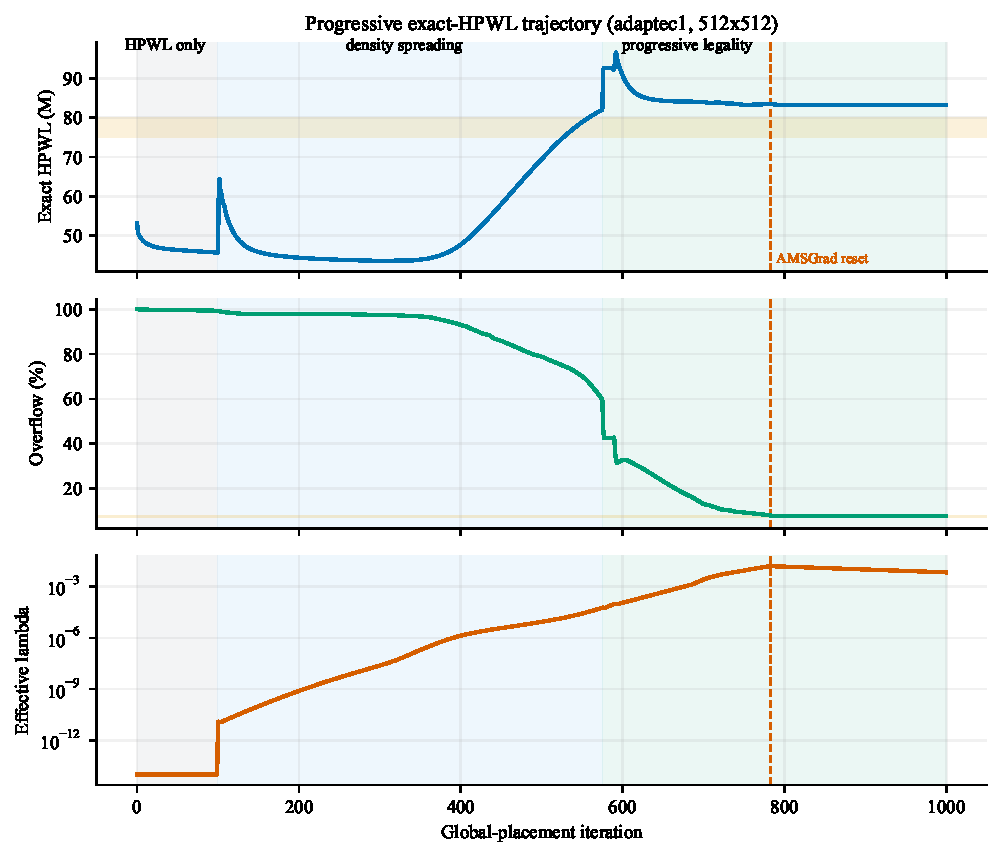
\includegraphics[width=0.94\textwidth]{fig_progressive_convergence.pdf}
\caption{最佳 512$\times$512 运行的精确 HPWL、overflow 与有效 $\lambda$。灰色为 HPWL-only，蓝色为静电展开，绿色为渐进合法化；虚线表示 AMSGrad 重启。}
\label{fig:convergence}
\end{figure}

图~\ref{fig:convergence} 显示，HPWL-only 阶段留下接近 $100\%$ overflow 的极密状态。阶段二在第 316 步附近达到全程最低 $43.588$M，但 overflow 仍约 $97.3\%$，没有可比意义。真正进入目标带时，空间展开已经把 HPWL 提高到约 $83.5$M。

\begin{figure}[H]
\centering
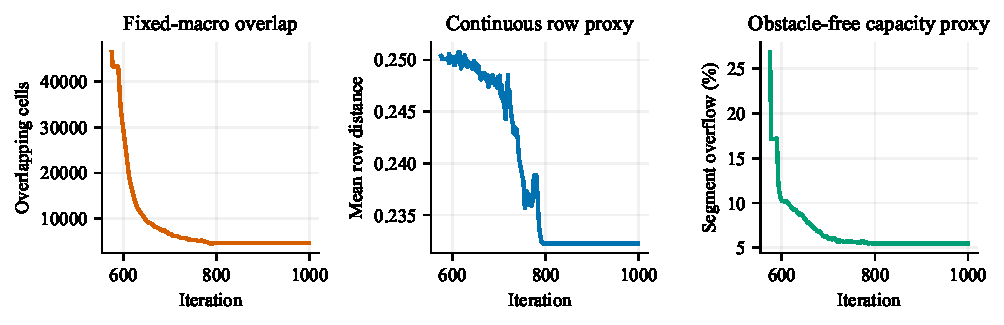
\includegraphics[width=0.96\textwidth]{fig_legality_proxies.pdf}
\caption{阶段三的连续合法性代理。宏重叠 cell 数、平均 row 距离和 segment overflow 均下降，但这些量不代替最终离散合法性检查。}
\label{fig:proxies}
\end{figure}

\begin{table}[H]
\centering
\small
\caption{adaptec1 消融。HPWL 单位为 M。}
\label{tab:ablation}
\begin{tabular}{lrrrrl}
\toprule
配置 & 网格/步数 & GP HPWL & Overflow & 合法 HPWL & 结论\\
\midrule
旧 exact Adam+bundle & 512/800 & 85.401 & 6.958\% & 91.030 & 旧基线\\
Pure BandDual & 512/800 & 101.277 & 7.266\% & 106.415 & 拒绝\\
Hybrid & 512/800 & 83.701 & 7.530\% & 89.237 & 有效\\
Hybrid+refine & 512/1000 & \textbf{83.254} & 7.744\% & \textbf{88.895} & 当前最佳\\
Sampling+bundle & 512/1000 & 83.577 & 7.741\% & 89.186 & 略差\\
\bottomrule
\end{tabular}
\end{table}

\begin{figure}[H]
\centering
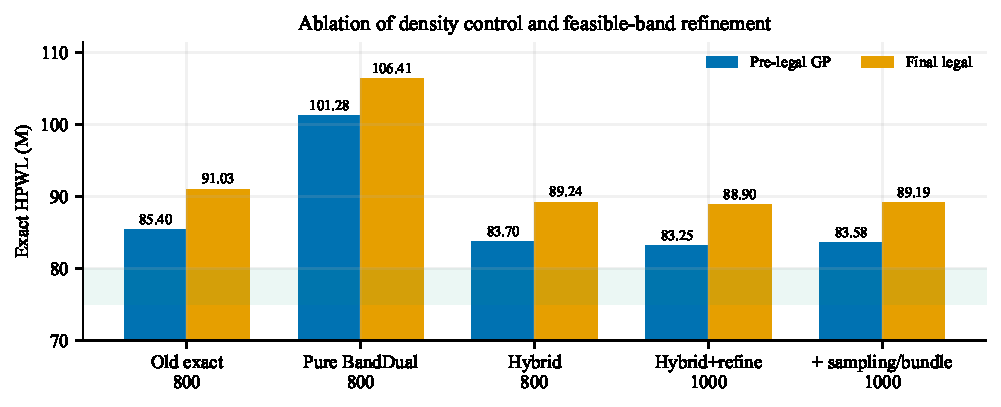
\includegraphics[width=0.94\textwidth]{fig_ablation.pdf}
\caption{混合 lambda 显著优于从高 overflow 起直接使用 BandDual；当前 gradient sampling+bundle 组合没有超过 Adam/AMSGrad 对照。绿色区域是希望达到的 $75$--$80$M GP 范围。}
\label{fig:ablation}
\end{figure}

主结果的阶段分解为
\begin{equation}
83.254\mathrm{M}/7.744\%
\rightarrow 89.971\mathrm{M}\;(\mathrm{Greedy})
\rightarrow 90.181\mathrm{M}\;(\mathrm{Abacus})
\rightarrow 88.895\mathrm{M}\;(\mathrm{DP}).
\end{equation}
最终合法化相对 GP 增加 $5.641$M，约 $6.78\%$。外部 checker 的四类错误均为 0，因此最终结果是真正离散合法，而不只是 overflow 较低。

64$\times$64 的 matched 对照还显示，加入 segment force 后 segment-overflow 代理从 $38.89\%$ 降到 $30.89\%$，合法 HPWL 从 $125.489$M 改善到 $124.650$M；尽管 GP HPWL 有约 $0.198$M 回退，合法后仍净改善 $0.839$M。因此 segment 力是面向最终合法结果的有效代理项。

\section{Bundle 与 gradient sampling 的结果}

探索运行加入一个邻域精确次梯度样本和 serious/null bundle。它得到 $83.577$M/$7.741\%\rightarrow89.186$M，比最佳对照分别差 $0.323$M 和 $0.291$M。第 845 步后连续 null step 把 trial scale 压到 0.01，预测下降趋于零。

这个负结果不等价于“bundle 不适合 HPWL”。当前全局 bundle 的 cut 同时包含大量网络的极值组合，而密度权重和活跃极值又持续变化；少量全局 cut 很快过时。相反，合法后的固定拓扑 bundle 已在独立实验中获得约 94.6K 的净改善。bundle 更适合以下两类 master：
\begin{enumerate}[nosep]
\item 合法前：逐网或分组 cut，加上密度约束的局部线性化，求密度切空间内的 trust-region 方向；
\item 合法后：固定 row、segment 和顺序，在明确凸多面体内求精确 HPWL epigraph/bundle 子问题。
\end{enumerate}

\section{为什么仍未达到 75--80M}

第一，100 步 HPWL-only 虽符合实验设想，却把 overflow 保持在约 $99.4\%$，相当于先制造一个极端中心团簇。阶段二必须重新建立二维拓扑，因此第 316 步的 $43.588$M 并不是可保留的好解。

第二，精确 HPWL 的单次次梯度非常稀疏。大网络只有当前左右上下极值 pin 获得力，绝大多数内部 pin 不参与该网络方向；在密度展开时，电场主导内部 cell，而线长模型无法提供平滑拓扑约束。

第三，lambda 只能调节两类梯度的幅值，无法处理它们的方向冲突。达到目标带以后，最需要的是“在 overflow 一阶不增的切空间中下降 HPWL”；标量权重与逐步回溯容易把所有 trial 都拒绝。第 799 步后的冻结就是直接证据。

第四，连续 row/segment 代理降低了离散合法化冲击，但当前宏重叠 cell 仍有 4557 个。最终合法化仍需一次有限的拓扑调整，产生 $5.641$M 的线长增量。

\section{下一步建议}

最优先的改进不是继续增加迭代，而是实现密度切空间的约束方向。令 $g_c$ 为 overflow 或密度违反的局部梯度，$d_H$ 为 gradient sampling 或分网 bundle 给出的 HPWL 方向，可求
\begin{equation}
\min_d\;\max_j\{H_j+g_j^\top d\}+\frac{1}{2t}\|d\|^2,
\quad
\text{s.t. } g_c^\top d\leq \delta_c,
\quad \|d\|_\infty\leq\Delta.
\end{equation}
当 overflow 已在带内时，$\delta_c$ 取 0 或很小的正数；超过上界时取负值。这比继续调一个 lambda 更直接地利用可行边界。

第二，应在阶段一中加入很弱但非零的密度 trust region，或把 HPWL-only 缩短到 75 步并限制局部容量恶化。该密度项不改变 HPWL 的非光滑定义，只防止形成必须完全重建的中心团簇。

第三，可把 $\varepsilon$-active set 和 gradient sampling 仅用于 trial direction，并仍由精确 HPWL/overflow filter 接受。对接近包围盒边界的内部 pin 分配方向，可以缓解极值切换和稀疏梯度问题。

第四，阶段三应把宏重叠 cell 数纳入 checkpoint 选择，并根据局部 segment 拥塞自适应放大障碍 ramp，而不是只使用全局固定系数。合法化时还可以合法化多个低重叠 checkpoint，再按最终 HPWL 选择。

\section{可回退性与验证}

所有新逻辑由 \code{--progressive-legalization} 控制。关闭该开关时，原 smooth DREAMPlace 路径、旧 exact 路径、命令格式和非 progressive CSV 表头保持不变。新增全局布局实现主要位于 \code{src/nonsmooth.cpp} 和 \code{src/obstacle.cpp}。Greedy/Abacus 与合法后算子仍复用 \code{src/legalizer.cpp}。

项目使用 MinGW C++17 完整重编译，\code{core_test} 通过且无编译警告。最佳 \code{final.pl} 经数据集自带 checker 验证：Type 0（固定对象移动）、Type 1（越界）、Type 2（行/站点不对齐）、Type 3（重叠）均为 0。实验数据、快照和指标位于 \code{output/progressive_a1_512_1000_refine}，可复现实验协议位于 \code{experiments/progressive-legalization/protocol.md}。

\section{结论}

本轮实现证明了“连续合法化再离散合法化”比直接粗暴移动更合理：最终合法化冲击被控制在 $5.641$M，且新流程优于旧的中心初始化精确 HPWL 基线。然而 $83.254$M 仍高于希望的 $75$--$80$M。数据不支持继续沿当前参数简单增加迭代，也不支持 pure BandDual 或当前全局 bundle。下一阶段应把问题从“继续调 lambda”提升为“显式求密度约束切空间中的非光滑 HPWL 方向”，并在极密阶段避免破坏二维拓扑。

\end{document}
